% =============================================================================
% CAPÍTULO 2 - BLOQUE 2.7: BASES DE DATOS VECTORIALES, MÉTRICAS DE EVALUACIÓN
% EMPÍRICA (RAGAS/ALCE) Y METODOLOGÍA DE REVISIÓN SISTEMÁTICA DE LITERATURA
% =============================================================================

\subsection{Bases de Datos Vectoriales, Evaluación Empírica y Metodología de Revisión}
\label{subsec:bases_datos_metricas}

\subsubsection{Arquitectura de Bases de Datos Vectoriales e Indexación HNSW}
\label{subsubsec:bases_datos_vectoriales_hnsw}

Una vez que los fragmentos de vídeo y las consultas en lenguaje natural han sido transformados en representaciones vectoriales densas por los modelos fundacionales, el sistema requiere una infraestructura de almacenamiento persistente capaz de indexar y recuperar alta dimensionalidad en tiempo real \cite{gemini_emb2_docs, qwen3_vl_emb2026}. %[cite: 2, 4]
En el estado del arte de 2026, motores especializados como \textbf{Qdrant}, \textbf{Milvus}, \textbf{Weaviate} y \textbf{Pinecone} se han consolidado como el estándar industrial para la gestión de repositorios vectoriales \cite{gemini_emb2_docs}. %[cite: 2]

En despliegues basados en motores como Qdrant, cada fragmento vectorizado se encapsula y almacena como una estructura de punto indexado (\texttt{PointStruct}) compuesta por tres elementos fundamentales \cite{gemini_emb2_docs}: %[cite: 2]
\begin{enumerate}
    \item \textbf{Identificador Único Determinista (UUIDv5):} Generado de forma unívoca a partir del nombre del archivo de vídeo y del índice secuencial del fragmento, lo que garantiza que reinsertar el mismo \texttt{VideoChunk} sobrescriba de manera idempotente su entrada anterior sin duplicar registros en la base de datos \cite{gemini_emb2_docs}. %[cite: 2]
    \item \textbf{Vector Denso ($\mathbf{v} \in \mathbb{R}^d$):} El tensor numérico de salida devuelto por el modelo (por ejemplo, configurado a $3.072$ dimensiones en \textit{Gemini Embedding 2} o $768$ dimensiones con normalización $L_2$), indexado mediante métrica de distancia coseno (\texttt{models.Distance.COSINE}) sobre grafos de mundos pequeños jerárquicos (\textit{Hierarchical Navigable Small World}, \textbf{HNSW}) \cite{gemini_emb2_docs}. %[cite: 2]
    \item \textbf{Carga Útil de Metadatos (\textit{Payload}):} Un diccionario estructurado adjunto al vector que almacena los atributos relacionales indispensables para la reconstrucción temporal del resultado, incluyendo el nombre del fichero (\texttt{video\_name}), el índice del fragmento (\texttt{chunk\_index}) y los instantes exactos de inicio y fin expresados en segundos flotantes (\texttt{start\_time} y \texttt{end\_time}) \cite{gemini_emb2_docs}. %[cite: 2]
\end{enumerate}

La Figura~\ref{fig:qdrant_hnsw_payload} ilustra la arquitectura de almacenamiento y el direccionamiento mediante índices HNSW en Qdrant. %[cite: 2]

\begin{figure}[htbp]
\centering
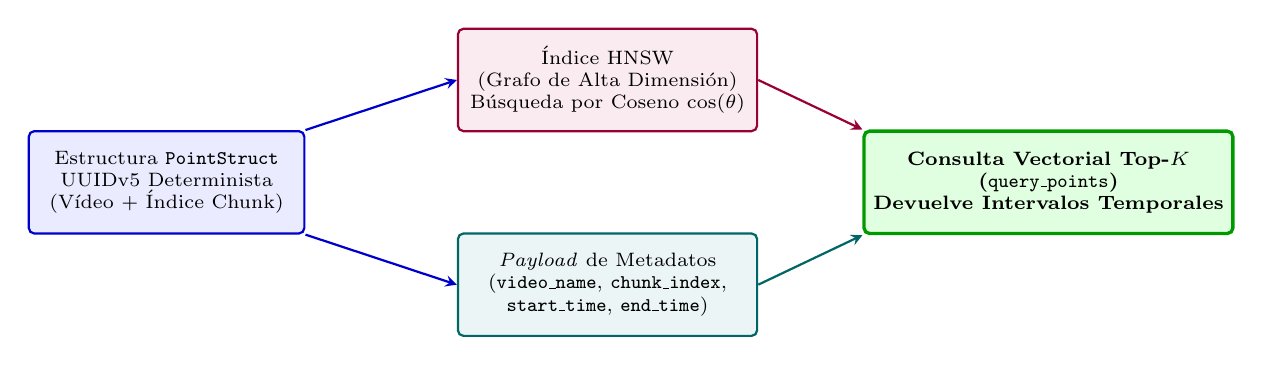
\begin{tikzpicture}[
    pointbox/.style={rectangle, draw=blue!80!black, fill=blue!8, thick, minimum width=3.5cm, minimum height=1.3cm, align=center, font=\scriptsize, rounded corners=2pt},
    hnswbox/.style={rectangle, draw=purple!80!black, fill=purple!8, thick, minimum width=3.8cm, minimum height=1.3cm, align=center, font=\scriptsize, rounded corners=2pt},
    payloadbox/.style={rectangle, draw=teal!80!black, fill=teal!8, thick, minimum width=3.8cm, minimum height=1.3cm, align=center, font=\scriptsize, rounded corners=2pt},
    outbox/.style={rectangle, draw=green!60!black, fill=green!12, very thick, minimum width=3.7cm, minimum height=1.3cm, align=center, font=\scriptsize\bfseries, rounded corners=2pt},
    arrow/.style={-stealth, thick, draw=black!80}
]
\node[pointbox] (point) at (-5.6, 0) {Estructura \texttt{PointStruct}\\UUIDv5 Determinista\\(Vídeo + Índice Chunk)};

\node[hnswbox] (hnsw) at (0, 1.3) {Índice HNSW\\(Grafo de Alta Dimensión)\\Búsqueda por Coseno $\cos(\theta)$};

\node[payloadbox] (payload) at (0, -1.3) {\textit{Payload} de Metadatos\\(\texttt{video\_name}, \texttt{chunk\_index},\\ \texttt{start\_time}, \texttt{end\_time})};

\node[outbox] (query) at (5.6, 0) {Consulta Vectorial Top-$K$\\(\texttt{query\_points})\\Devuelve Intervalos Temporales};

\draw[arrow, blue!80!black] (point.north east) -- (hnsw.west);
\draw[arrow, blue!80!black] (point.south east) -- (payload.west);
\draw[arrow, purple!80!black] (hnsw.east) -- (query.north west);
\draw[arrow, teal!80!black] (payload.east) -- (query.south west);
\end{tikzpicture}
\caption{Arquitectura de almacenamiento y recuperación en Qdrant: separación de vectores densos indexados mediante grafos HNSW y metadatos temporales alojados en el \textit{payload} para consultas top-$K$ ultra rápidas \cite{gemini_emb2_docs}.} %[cite: 2]
\label{fig:qdrant_hnsw_payload}
\end{figure}

\subsubsection{Métricas Clásicas de Recuperación y Bancos de Pruebas Masivos (MMEB-V2 y MVEB)}
\label{subsubsec:metricas_clasicas_benchmarks}

La validación empírica del rendimiento de los sistemas de recuperación de información multimedia se apoya en una combinación de métricas estadísticas clásicas y bancos de pruebas (\textit{benchmarks}) estandarizados a escala masiva \cite{qwen3_vl_emb2026, eval_mrag2025}. %[cite: 2, 4]

En primer lugar, las métricas clásicas de Recuperación de Información evalúan la precisión del ordenamiento top-$K$ devuelto por la base de datos vectorial frente a la verdad terreno (\textit{ground truth}) \cite{qwen3_vl_emb2026}: %[cite: 2, 4]
\begin{itemize}
    \item \textbf{\textit{Recall@K}:} Mide la proporción de fragmentos relevantes reales que han sido recuperados dentro de los primeros $K$ resultados devueltos \cite{qwen3_vl_emb2026}. %[cite: 2, 4]
    \item \textbf{\textit{Precision@K}:} Cuantifica qué porcentaje de los $K$ resultados devueltos por el sistema son efectivamente relevantes \cite{qwen3_vl_emb2026}. %[cite: 4]
    \item \textbf{\textit{Hit@1} (o \textit{Accuracy@1}):} Evalúa si el primer resultado devuelto por el motor de búsqueda coincide exactamente con el evento buscado \cite{qwen3_vl_emb2026}. %[cite: 4]
    \item \textbf{\textit{nDCG@K} (\textit{Normalized Discounted Cumulative Gain}):} Evalúa la calidad del ranking ponderando la posición de los aciertos, penalizando severamente cuando un resultado relevante aparece en posiciones inferiores de la lista \cite{qwen3_vl_emb2026}. %[cite: 2, 4]
\end{itemize}

A nivel global, la comunidad investigadora evalúa los modelos sobre dos bancos de pruebas masivos de referencia actualizados para 2026 \cite{qwen3_vl_emb2026}: %[cite: 2, 4]
\begin{enumerate}
    \item \textbf{MMEB-V2 (\textit{Massive Multimodal Embedding Benchmark V2}, 2025):} Consolida más de 78 conjuntos de datos para evaluar la recuperación conjunta sobre texto, imágenes, vídeo y documentos estructurados (PDF), estandarizando mediciones de \textit{Recall@1} y \textit{nDCG@5} \cite{qwen3_vl_emb2026}. %[cite: 2, 4]
    \item \textbf{MVEB (\textit{Massive Video Embedding Benchmark}, 2026):} El estándar específico más riguroso para la comprensión temporal de vídeo de larga duración, abarcando más de 180 tareas de recuperación cruzada entre pistas visuales y auditivas \cite{qwen3_vl_emb2026}. %[cite: 2, 4]
\end{enumerate}

\subsubsection{Frameworks de Evaluación RAG y Atribución Verificable (RAGAS, ALCE, ARGUE, MIRAGE)}
\label{subsubsec:frameworks_ragas_alce}

La evaluación de arquitecturas RAG multimodales exige ir más allá de la simple recuperación de vectores, analizando la calidad de la generación de respuestas y la veracidad de la atribución temporal \cite{eval_mrag2025, video_rac2025}. %[cite: 2, 4]
El marco de referencia contemporáneo se estructura en torno a dos metodologías complementarias \cite{eval_mrag2025, video_rac2025}: %[cite: 2, 4]

\paragraph{Framework RAGAS (\textit{Retrieval Augmented Generation Assessment}):}
Descompone la calidad de la respuesta generada por el modelo de lenguaje en tres dimensiones fundamentales independientes \cite{video_rac2025}: %[cite: 2, 4]
\begin{itemize}
    \item \textbf{\textit{Answer Relevance}:} Mide el grado de pertinencia y coherencia de la respuesta generada respecto a la consulta original del usuario \cite{video_rac2025}. %[cite: 2, 4]
    \item \textbf{\textit{Context Relevance}:} Evalúa la precisión del material recuperado por la base de datos vectorial, penalizando la inclusión de fragmentos de vídeo irrelevantes que aporten ruido al contexto \cite{video_rac2025}. %[cite: 2, 4]
    \item \textbf{\textit{Faithfulness} (Fidelidad):} Cuantifica si la respuesta generada se deriva estrictamente del contexto recuperado, detectando y penalizando cualquier alucinación o invención por parte del modelo \cite{video_rac2025}. %[cite: 2, 4]
\end{itemize}

\paragraph{Métricas de Atribución Verificable (ALCE, ARGUE, MIRAGE):}
Marcos como \textbf{ALCE} (\textit{Automatic LLM Citation Evaluation}), \textbf{ARGUE} y \textbf{MIRAGE} extienden la evaluación para auditar si cada afirmación generada en la respuesta cuenta con un enlace de citación directo y verificable hacia el intervalo temporal exacto ($[t_{\text{inicio}}, t_{\text{fin}}]$) del vídeo fuente, garantizando una trazabilidad forense inalterable \cite{eval_mrag2025}. %[cite: 2, 4]

La Figura~\ref{fig:frameworks_ragas_alce} resume la estructura jerárquica de evaluación mediante RAGAS y métricas de atribución verificable. %[cite: 2, 4]

\begin{figure}[htbp]
\centering
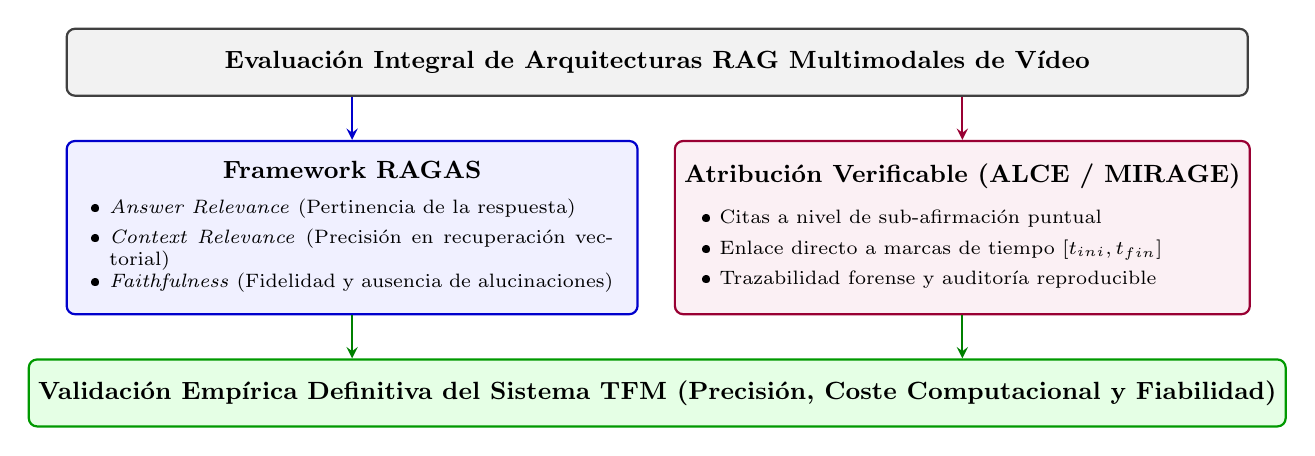
\begin{tikzpicture}[
    boxroot/.style={rectangle, draw=black!75, fill=gray!10, thick, minimum width=15.0cm, minimum height=0.85cm, align=center, font=\small\bfseries, rounded corners=3pt},
    boxcol1/.style={rectangle, draw=blue!80!black, fill=blue!6, thick, minimum width=7.25cm, minimum height=2.2cm, align=center, rounded corners=3pt},
    boxcol2/.style={rectangle, draw=purple!80!black, fill=purple!6, thick, minimum width=7.25cm, minimum height=2.2cm, align=center, rounded corners=3pt},
    boxout/.style={rectangle, draw=green!60!black, fill=green!10, thick, minimum width=15.0cm, minimum height=0.85cm, align=center, font=\small\bfseries, rounded corners=3pt},
    arrow/.style={-stealth, thick}
]
\node[boxroot] (root) at (0, 3.2) {Evaluación Integral de Arquitecturas RAG Multimodales de Vídeo};

\node[boxcol1] (rgs) at (-3.875, 1.1) {%
    {\bfseries\small Framework RAGAS}\\[6pt]
    \scriptsize
    \begin{tabular}{@{\textbullet~}p{6.4cm}@{}}
    \textit{Answer Relevance} (Pertinencia de la respuesta)\\[3pt]
    \textit{Context Relevance} (Precisión en recuperación vectorial)\\[3pt]
    \textit{Faithfulness} (Fidelidad y ausencia de alucinaciones)
    \end{tabular}
};

\node[boxcol2] (alc) at (3.875, 1.1) {%
    {\bfseries\small Atribución Verificable (ALCE / MIRAGE)}\\[6pt]
    \scriptsize
    \begin{tabular}{@{\textbullet~}p{6.4cm}@{}}
    Citas a nivel de sub-afirmación puntual\\[3pt]
    Enlace directo a marcas de tiempo $[t_{\text{ini}}, t_{\text{fin}}]$\\[3pt]
    Trazabilidad forense y auditoría reproducible
    \end{tabular}
};

\node[boxout] (out) at (0, -1.0) {Validación Empírica Definitiva del Sistema TFM (Precisión, Coste Computacional y Fiabilidad)};

\draw[arrow, blue!80!black] (root.south -| rgs.north) -- (rgs.north);
\draw[arrow, purple!80!black] (root.south -| alc.north) -- (alc.north);
\draw[arrow, green!50!black] (rgs.south) -- (out.north -| rgs.south);
\draw[arrow, green!50!black] (alc.south) -- (out.north -| alc.south);
\end{tikzpicture}
\caption{Estructura combinada de evaluación empírica mediante el framework RAGAS y métricas de atribución verificable (ALCE/MIRAGE) para validar el rendimiento del sistema RAG de vídeo \cite{eval_mrag2025, video_rac2025}.} %[cite: 2, 4]
\label{fig:frameworks_ragas_alce}
\end{figure}

\subsubsection{Metodología de Revisión Sistemática de la Literatura Asistida por NotebookLM}
\label{subsubsec:metodologia_revision_notebooklm}

Para llevar a cabo la recopilación, filtrado y síntesis crítica de las fuentes bibliográficas empleadas a lo largo de este estado del arte, la investigación ha adoptado un marco metodológico estructurado en un \textbf{flujo de trabajo de cuatro etapas asistido por entornos RAG acotados y gestores bibliográficos} (tales como Zotero sincronizado con repositorios abiertos en arXiv) \cite{easton2026notebooklm, sourclip2026notebooklm}: %[cite: 2, 4]

\begin{enumerate}
    \item \textbf{Etapa 1 - Construcción y Depuración de la Base de Conocimiento Acotada:} Recopilación sistemática de artículos preprints y documentación técnica cumpliendo restricciones operativas (tales como los límites de ingestión de 50 fuentes por cuaderno y 500.000 palabras por documento en herramientas como Google NotebookLM), resolviéndolo mediante la fusión temática de artículos o el uso de múltiples cuadernos especializados \cite{easton2026notebooklm}. %[cite: 2, 4]
    \item \textbf{Etapa 2 - Síntesis Estructural y Descubrimiento Topológico:} Análisis automatizado de convergencia tecnológica mediante resúmenes fonéticos integrados (\textit{Audio Overview}) y generación de cronologías de evolución arquitectónica \cite{easton2026notebooklm, sourclip2026notebooklm}. %[cite: 2, 4]
    \item \textbf{Etapa 3 - Análisis Crítico, Deconstrucción Metodológica y Lazo de Relleno de Brechas (\textit{Gap-Fill Loop}):} Contraste sistemático de hipótesis metodológicas y detección de vacíos en la literatura previa sobre fragmentación adaptativa y modelos multimodales \cite{easton2026notebooklm}. %[cite: 2, 4]
    \item \textbf{Etapa 4 - Verificación Transparente y Consolidación Causal:} Auditoría inalienable de las citas generadas contrastándolas directamente sobre los textos fuente originales para garantizar la ausencia de alucinaciones teóricas en la memoria del TFM \cite{easton2026notebooklm, sourclip2026notebooklm}. %[cite: 2, 4]
\end{enumerate}

La Figura~\ref{fig:flujo_cuatro_etapas_literatura} esquematiza este flujo metodológico de investigación sistemática. %[cite: 2, 4]

\begin{figure}[htbp]
\centering
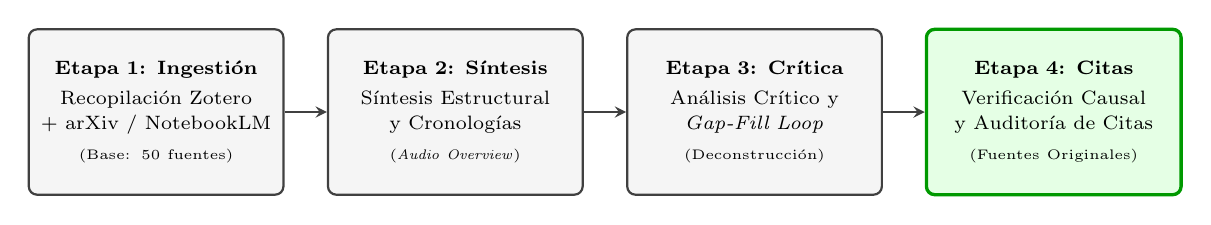
\begin{tikzpicture}[
    stepbox/.style={rectangle, draw=black!75, fill=gray!8, thick, text width=3.0cm, minimum height=2.1cm, align=center, font=\scriptsize, rounded corners=3pt},
    outbox/.style={rectangle, draw=green!60!black, fill=green!10, very thick, text width=3.0cm, minimum height=2.1cm, align=center, font=\scriptsize, rounded corners=3pt},
    arrow/.style={-stealth, thick, draw=black!75}
]
\node[stepbox] (s1) at (-5.7, 0) {\textbf{Etapa 1: Ingestión}\\[3pt]Recopilación Zotero\\[1pt]+ arXiv / NotebookLM\\[3pt]{\normalfont\tiny (Base: 50 fuentes)}};
\node[stepbox] (s2) at (-1.9, 0) {\textbf{Etapa 2: Síntesis}\\[3pt]Síntesis Estructural\\[1pt]y Cronologías\\[3pt]{\normalfont\tiny (\textit{Audio Overview})}};
\node[stepbox] (s3) at (1.9, 0) {\textbf{Etapa 3: Crítica}\\[3pt]Análisis Crítico y\\[1pt]\textit{Gap-Fill Loop}\\[3pt]{\normalfont\tiny (Deconstrucción)}};
\node[outbox] (s4) at (5.7, 0) {\textbf{Etapa 4: Citas}\\[3pt]Verificación Causal\\[1pt]y Auditoría de Citas\\[3pt]{\normalfont\tiny (Fuentes Originales)}};

\draw[arrow] (s1) -- (s2);
\draw[arrow] (s2) -- (s3);
\draw[arrow] (s3) -- (s4);
\end{tikzpicture}
\caption{Flujo metodológico de cuatro etapas para la revisión sistemática de la literatura apoyado en gestores bibliográficos y entornos RAG acotados \cite{easton2026notebooklm, sourclip2026notebooklm}.} %[cite: 2, 4]
\label{fig:flujo_cuatro_etapas_literatura}
\end{figure}

El Cuadro~\ref{tab:resumen_metodologia_evaluacion} consolida las métricas, frameworks y metodologías de evaluación y revisión analizadas en este último bloque del estado del arte. %[cite: 2, 4]

\begin{table}[htbp]
\centering
\small
\setlength{\tabcolsep}{4.5pt}
\caption{Síntesis de métricas, bancos de pruebas y metodologías de evaluación en sistemas Video RAG \cite{qwen3_vl_emb2026, eval_mrag2025, video_rac2025, easton2026notebooklm}.} %[cite: 2, 4]
\label{tab:resumen_metodologia_evaluacion}
\begin{tabularx}{\linewidth}{>{\raggedright\arraybackslash}p{3.4cm} >{\raggedright\arraybackslash}p{3.2cm} >{\raggedright\arraybackslash}p{3.8cm} >{\raggedright\arraybackslash}X}
\toprule
\textbf{Categoría} & \textbf{Framework} & \textbf{Métricas} & \textbf{Objetivo en el TFM} \\
\midrule
Recuperación Vectorial & Qdrant + HNSW & \textit{Recall@K}, \textit{Hit@1}, \textit{nDCG@5} & Eficacia en la localización top-$K$ \\
Benchmarks Masivos & MMEB-V2 / MVEB & Recuperación multicanal & Comparativa con estándares 2026 \\
Calidad RAG y Fidelidad & Framework RAGAS & \textit{Answer/Context Rel.}, \textit{Faithfulness} & Evaluación de alucinaciones y contexto \\
Atribución Verificable & ALCE / MIRAGE & Citas a nivel de afirmación & Trazabilidad temporal en milisegundos \\
Revisión Bibliográfica & Zotero + NotebookLM & Flujo 4 etapas + \textit{Gap-Fill} & Rigor metodológico y estado del arte \\
\bottomrule
\end{tabularx}
\end{table}